\documentclass[letterpaper]{article}

%% Language and font encodings
\usepackage[english]{babel}
\usepackage[utf8x]{inputenc}
\usepackage[T1]{fontenc}

%% Sets page size and margins
\usepackage[letterpaper,top=3cm,bottom=2cm,left=2cm,right=2cm,marginparwidth=1.75cm]{geometry}

%% Useful packages
\usepackage{amsmath}
\usepackage{graphicx}
\usepackage[colorinlistoftodos]{todonotes}
\usepackage[colorlinks=true, allcolors=blue]{hyperref}
\usepackage{mathtools}
\usepackage{latexsym}
\usepackage{matlab-prettifier}

\title{Speech Processing HW5}
\author{Matt Ruffner}

\lstset{
  style              = Matlab-editor,
  basicstyle         = \mlttfamily,
  escapechar         = ",
  mlshowsectionrules = true,
}

\begin{document}

\maketitle

\section{Speaker Identification}
From the MSR Identity Toolbox:

\begin{lstlisting}[caption = {GMM-UBM Training Code from THe MSR Toolbox.}]

rng('default')
% Step1: Create the universal background model from all the
% training speaker data
nmix = nMixtures; % In this case, we know the # of mixtures needed
final_niter = 10;
ds_factor = 1;
ubm = gmm_em(trainSpeakerData(:), nmix, final_niter, ds_factor, ...
nWorkers);
%%
% Step2: Now adapt the UBM to each speaker to create GMM speaker model.
map_tau = 10.0;
config = 'mwv';
gmm = cell(nSpeakers, 1);
for s=1:nSpeakers
 gmm{s} = mapAdapt(trainSpeakerData(s, :), ubm, map_tau, config);
end
%%
% Step3: Now calculate the score for each model versus each speaker's
% data.
% Generate a list that tests each model (first column) against all the
% testSpeakerData.
trials = zeros(nSpeakers*nChannels*nSpeakers, 2);
answers = zeros(nSpeakers*nChannels*nSpeakers, 1);
for ix = 1 : nSpeakers,
 b = (ix-1)*nSpeakers*nChannels + 1;
 e = b + nSpeakers*nChannels - 1;
 trials(b:e, :) = [ix * ones(nSpeakers*nChannels, 1), ...
(1:nSpeakers*nChannels)'];
 answers((ix-1)*nChannels+b : (ix-1)*nChannels+b+nChannels-1) = 1;
 end
gmmScores = score_gmm_trials(gmm, reshape(testSpeakerData', ...
nSpeakers*nChannels,1), trials, ubm);
%%
% Step4: Now compute the EER and plot the DET curve and confusion matrix
imagesc(reshape(gmmScores,nSpeakers*nChannels, nSpeakers))
title('Speaker Verification Likelihood (GMM Model)');
ylabel('Test # (Channel x Speaker)'); xlabel('Model #');
colorbar; drawnow; axis xy
figure
eer = compute_eer(gmmScores, answers, false);

\end{lstlisting}

\section{Speech Coding}


\section{Speech Synthesis}
Using the \texttt{sapisynth} command from the Voicebox toolbox in MATLAB, the following sentence was synthesized:
\begin{quote}
    Oh my god can I pet your dog?
\end{quote}

The code to implement this, with a female child voice spoken 3 increments faster and the pitch shifted up by 3, with the word dog emphasized, is shown below:

\begin{lstlisting}[caption = {Sentence of speech that was synthesized.}]
>> sapisynth('<rate speed="3">Oh my god can i pet your <emph>dog?</emph></rate>','fcp3')

\end{lstlisting}

The Spectrogram of the synthesized speech is shown in Fig. \ref{fig:spec}.

\begin{figure}[h!]
    \centering
    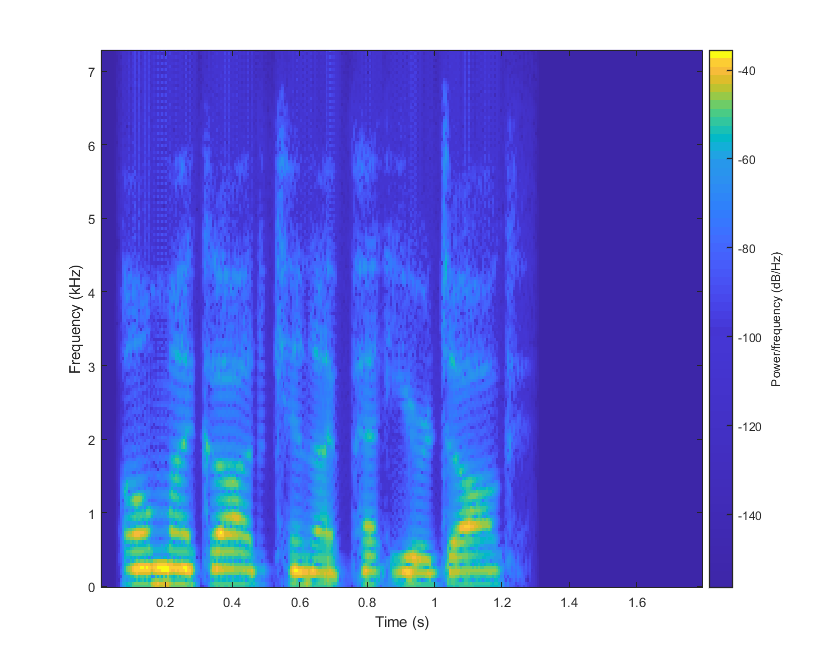
\includegraphics[width=10cm]{ee599hw5p3}
    \caption{Spectrogram of synthesized speech.}
    \label{fig:spec}
\end{figure}


%%%%%%%%%%%%%%%%%%%%%%%%%%%%%%%%%%%%%%%%%%%%%%%%%%%%
%%%%%%%%%%%%%%%%%%%%%%%%%%%%%%%%%%%%%%%%%%%%%%%%%%%%
%%%%%%%%%%%%%%%%%%%%%%%%%%%%%%%%%%%%%%%%%%%%%%%%%%%%
\section{Speech Enhancement}

The code for this is shown in Listing \ref{pt4code}.

\lstinputlisting[caption = {Code for speech enhancement using\texttt{ssubmmse}.}]{hw5p4.m}

\bibliographystyle{ieeetr}
\bibliography{refs.bib}
\end{document}